\documentclass{beamer}

\usepackage[utf8]{inputenc}
\usepackage{svg}
\usepackage{graphicx}
\usepackage{lmodern}

\usetheme{AnnArbor}
\usecolortheme{beaver}

\begin{document}

\title{Bioinformatics of the Immune System}
\author{Lasath Fernando}

\begin{frame}
\titlepage
\end{frame}

\section{Background}
\begin{frame}
  \frametitle{Immunoglobulins}

  \begin{columns}
    \begin{column}{5cm}
    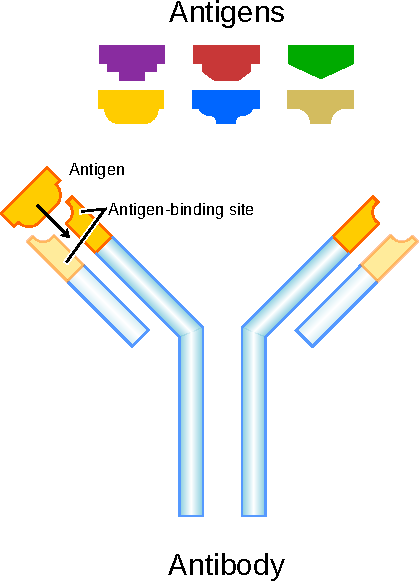
\includegraphics[width=\textwidth]{antibody.pdf}
    \end{column}
    \begin{column}{5cm}
    \begin{itemize}
     \item Also known as antibodies
     \item Y-shaped protien
     \item Has two purposes
     \begin{itemize}
      \item T
     \end{itemize}

     \item Produced by B-Cells
    \end{itemize}

    \end{column}
  \end{columns}

\end{frame}

\begin{frame}
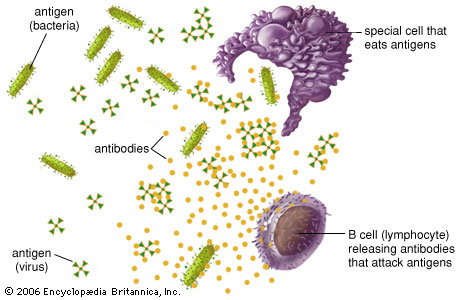
\includegraphics[width=\textwidth]{antigens-antibodies.jpg}
\end{frame}

\section{Motivation}
\section{Existing Strucutre}
\section{Plan}

\end{document}
